\documentclass[english,compress,handout]{beamer}

%\includeonlyframes{current}

\usepackage[ngerman]{babel}
\usepackage[T1]{fontenc}
\usepackage{graphicx}
\usepackage[utf8]{inputenc}
\usepackage{lmodern}
\usepackage{url}

\title{Krautspace}
\subtitle{Der Hackerspace in Jena}
\author[Schöbel]{Konrad \& Frank}
\institute[Hackspace Jena]{Hackspace Jena}
\date[23/10/2012]{Fachhochschule Jena \\ 23. Oktober 2012}

\subject{Hackerspaces}
\keywords{Hackerspaces Jena}

\usetheme{Boadilla}
\useinnertheme[shadow]{rounded}
\useoutertheme{split}
\usecolortheme{beetle}
\usefonttheme{structuresmallcapsserif}

\setbeamertemplate{headline}[infolines theme]
\setbeamertemplate{footline}[default]
\setbeamertemplate{navigation symbols}{}
\setbeamertemplate{frametitle}[default][right]

\setbeamercovered{dynamic}
\AtBeginSection[]
{
%	\begin{frame}
%		\tableofcontents[currentsection,hideallsubsections]
%	\end{frame}
}

\begin{document}

\begin{center}

\begin{frame}
	\titlepage
\end{frame}

\begin{frame}
	\Large Hackerspace \quad = \quad Hacker \quad + \quad Space
\end{frame}

%------------------------------------------------------------------------------------------------------------------------------%
\section{Was ist ein Hacker?}

\begin{frame}
	\frametitle{Ein Hacker ist \ldots}
	\begin{itemize}
		\item \ldots ein Tüftler, der bekannte Sachen auseinandernimmt, \\
			versteht und neu zusammen setzt. \bigskip\\
		\item \ldots jemand, der Spaß an kreativem Umgang mit Technik hat.
	\end{itemize}
\end{frame}

%------------------------------------------------------------------------------------------------------------------------------%
\section{Was ist ein Hackerspace?}

\begin{frame}
	\frametitle{Ein Hackerspace ist \ldots}
	\vfill
	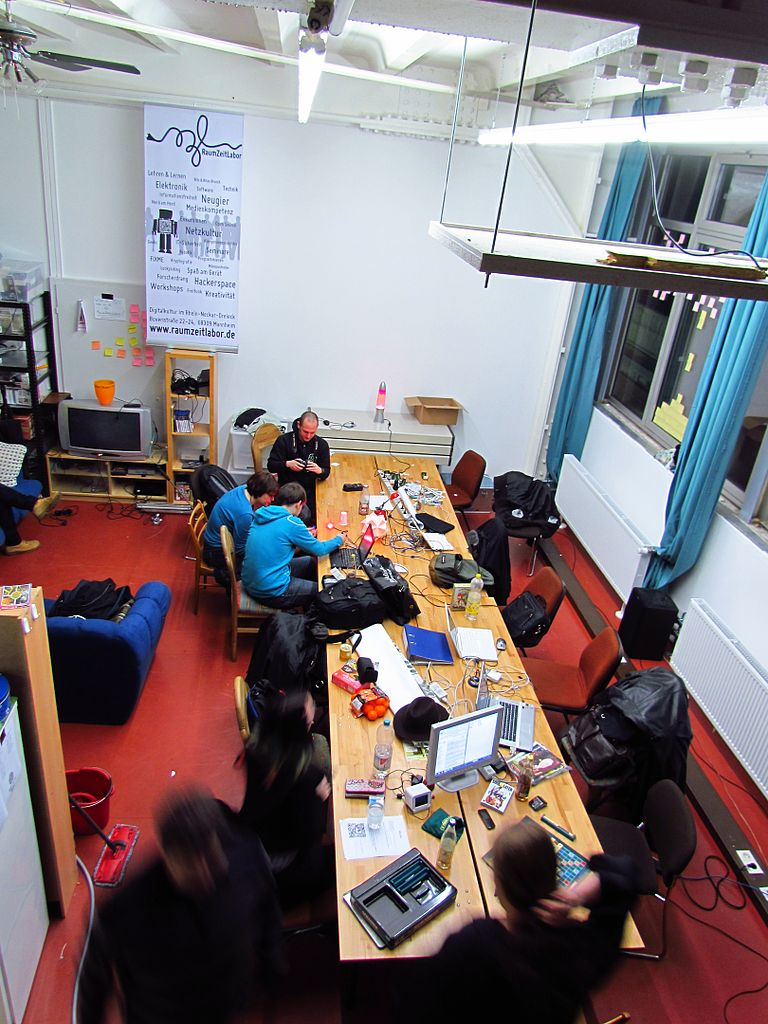
\includegraphics[height=.625\textheight]{media/Raumzeitlabor}
	\vfill
	\ldots ein physischer Raum für Hacker.\\
	\hfill
	\tiny{Foto: Raumzeitlabor}
\end{frame}

\begin{frame}
	\frametitle{Ein Hackerspace ist \ldots}
	\ldots ein offener Raum.
\end{frame}

\begin{frame}
	\frametitle{Ein Hackerspace ist \ldots}
	\ldots ein "`Infrastrukturprovider"':
	\vfill
	\begin{itemize}
		\item Raum
		\item Strom
		\item Internet
		\item Kontakte
		\item Werkzeuge und Bauteile
		\item Essen \& Trinken
	\end{itemize}
\end{frame}

\begin{frame}
	\frametitle{In einem Hackerspace gibt es \ldots}
	\begin{itemize}
		\item Do-It-Yourself
		\item Vorträge
		\item Workshops
		\item Diskussionen
		\item zocken
		\item Parties
	\end{itemize}
	\pause
	\vfill
    Themen:
	\vfill
	\begin{itemize}
		\item Hardware
		\item Software
		\item Gesellschaft \& Technologie
		\item Kunst
	\end{itemize}
\end{frame}

\begin{frame}
	\frametitle{Veranstaltungen}
	\framesubtitle{Rückblick}
	\begin{itemize}
		\item Anfang Oktober: Hackerfahrschule 
			\begin{itemize}
				\item Linux
				\item Shell
				\item vi vs emacs
				\item \LaTeX{}
				\item Tor
				\item git
			\end{itemize}
		\item DIY Kochrunden (Nudeln, Chili)
	\end{itemize}
\end{frame}

\begin{frame}
	\frametitle{Veranstaltungen}
	\framesubtitle{Voraussschau}
	\begin{itemize}
		\item regelmäßig:
			\begin{itemize}
				\item dienstags: offene Runde mit \texttt{0xAFFE}
				\item jeden zweiten Donnerstag: Stammtisch der LUG Jena
				\item jeden zweiten Sonntag: Chaoscafe
			\end{itemize}
		\item 24. Oktober: Einführung in Gentoo-Linux
		\item 15. November: Vortrag von Matthias Kirschner (FSFE):  \\
			\begin{quote}
				\textit{Vom Aussterben bedroht: Die Universalmaschine Computer}
			\end{quote}
		\item Deine Idee hier!
	\end{itemize}	
\end{frame}

\begin{frame}
	\frametitle{Ein Hackerspace \ldots}
	\ldots lebt von seinen Mitgliedern.
\end{frame}


%------------------------------------------------------------------------------------------------------------------------------%
\section{Der Jenaer Hackspace}

\begin{frame}
	\frametitle{Der Krautspace}
	\framesubtitle{real}
	\hspace*{\fill}
	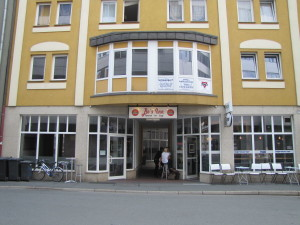
\includegraphics[width=5cm]{media/durchgang_zum_space.jpg}
	\hfill
	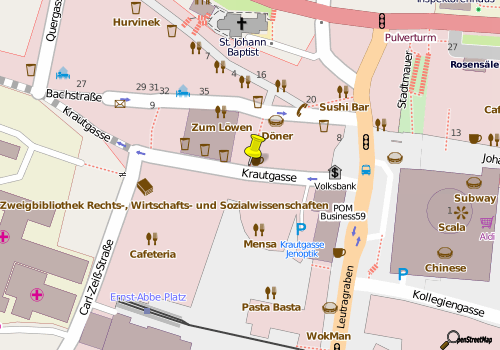
\includegraphics[width=5cm]{media/oss_location.png}
	\hspace*{\fill}
	\bigskip\\
	Krautgasse 26
\end{frame}

\begin{frame}
	\frametitle{Der Krautspace}
	\framesubtitle{virtuell}
	\begin{center}
		\begin{tabular}{ll}
			Homepage & \url{http://www.krautspace.de}\\
			Mailingliste & \url{http://yaturl.net/0d3a}\\
			Jabber & \url{xmpp://hackspace@chat.lug-jena.de}\\
			Twitter & \url{@HackspaceJena}\\
			identi.ca & \url{@HackspaceJena}\\
			\\
			& \url{www.hackerspaces.org}\\
		\end{tabular}
	\end{center}
\end{frame}

\end{center}

\end{document}

vim:  textwidth=128  nowrap  shiftwidth=4  spelllang=de  nofoldenable
